Using Canvas, you are to draw vectors. For this,
\begin{enumerate}
\item Make a function
  \begin{quote}
    \mbox{\lstinline! toInt: vec -> int * int!}
  \end{quote}
  which takes a vector of floats and returns a vector of ints.
\item Using \lstinline{add} and \lstinline{toInt}, make a function
  \begin{quote}
    \mbox{\lstinline! setVector: canvas -> color -> vec -> vec -> unit!}
  \end{quote}
  which takes a canvas, a color, a vector \lstinline{v}, and a position \lstinline{p} and draws a line from \lstinline{p} to \lstinline{p+v} using \lstinline{setLine}. Demonstrate that this works by creating a horizontal vector with its tail at the center of the canvas, and show it on screen using \lstinline{show}.
\item Using \lstinline{rot} and \lstinline{setVector} make a function
  \begin{quote}
    \mbox{\lstinline! draw: int -> int -> canvas!}
  \end{quote}
  which creates a canvas with a given width and height, adds 36 spokes as illustrated in \Cref{fig:spokes}, and returns the canvas.
  \begin{figure}
    \centering
    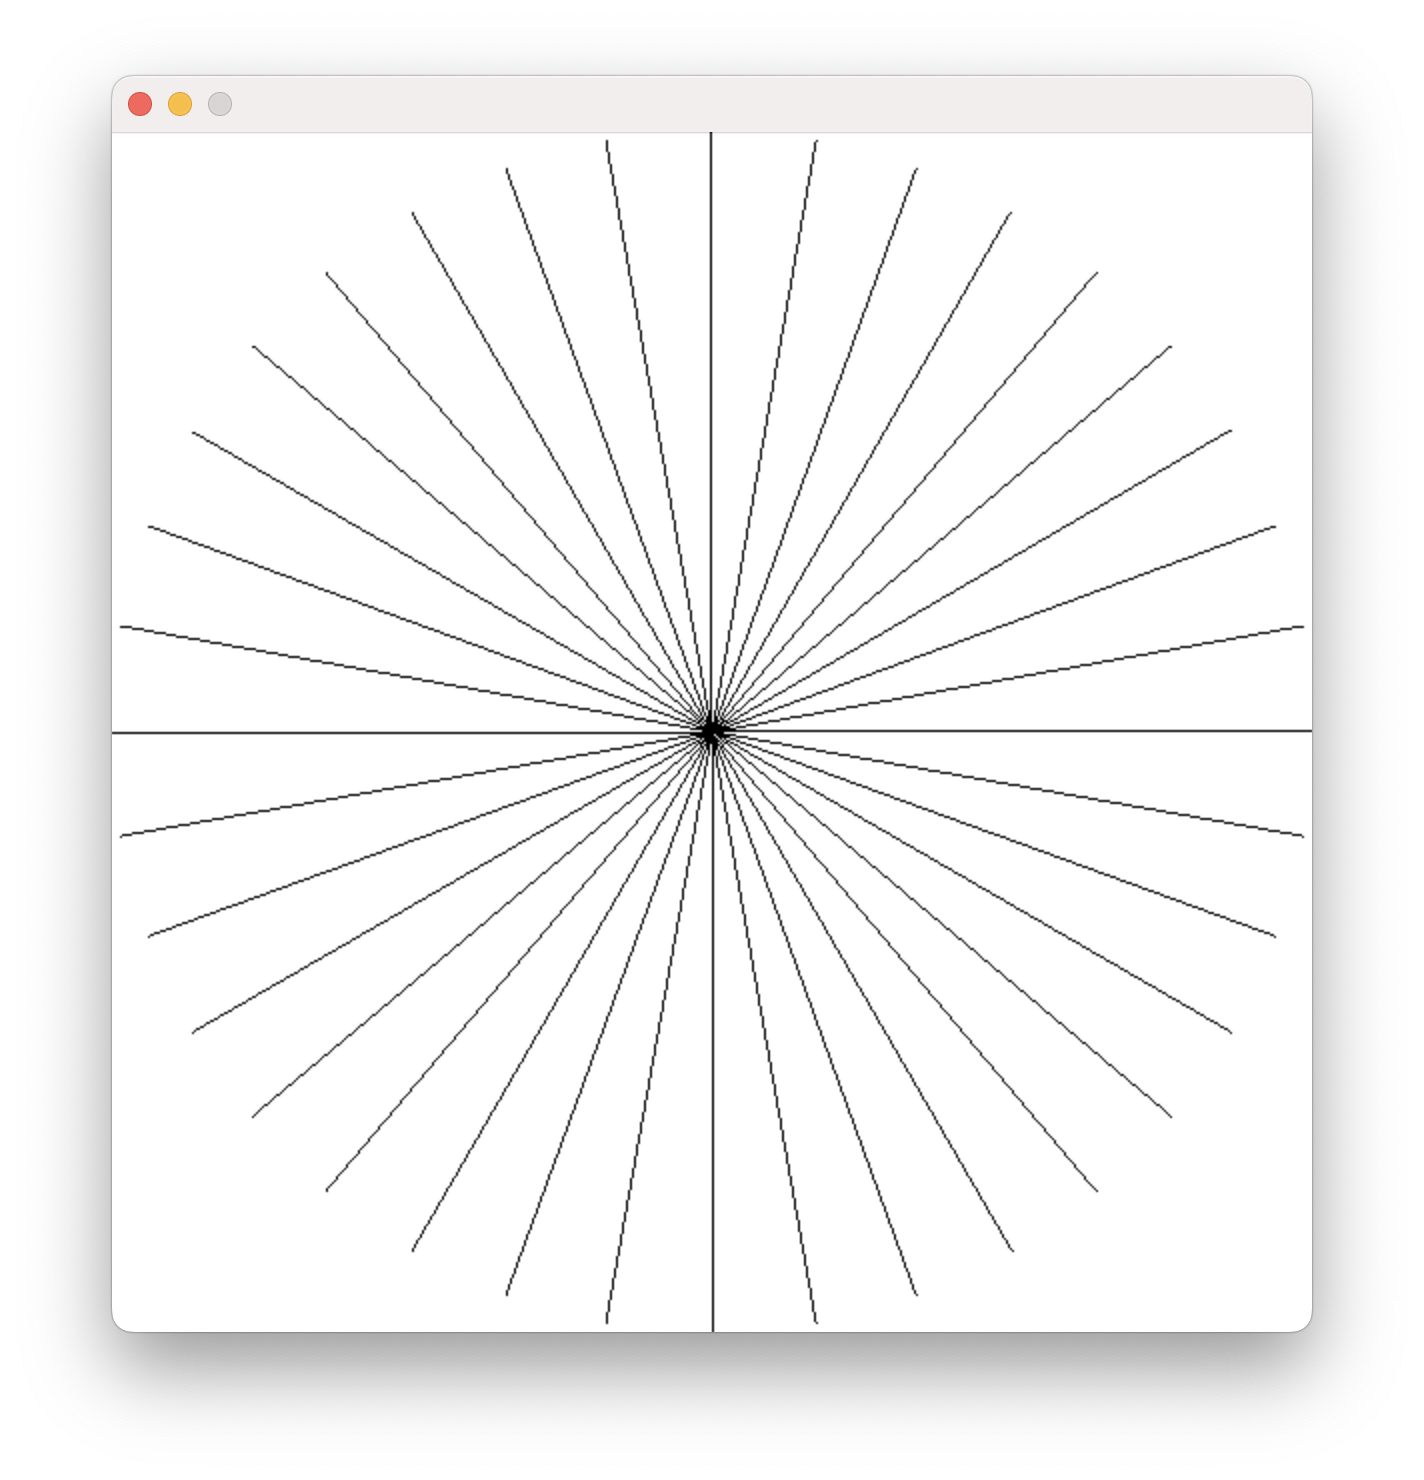
\includegraphics[width=0.4\textwidth]{spokes}
    \caption{36 radial lines from the center of a canvas.}
    \label{fig:spokes}
  \end{figure}
  Demonstrate that this works by showing the canvas on screen with \lstinline{show}.
\item Optional: Use these in \lstinline{runApp} to make an interactively rotating set of spokes as follows: Extend \lstinline{draw} with a float state parameter \lstinline{s}, which draws the spokes with the angular offset \lstinline{s}. Add a reaction function \lstinline{react} which changes the offset by $\pm0.01$ when the right and left arrow key are pressed respectively.
\end{enumerate}
The functions are to be documented using the \verb|<summary>|, \verb|<param>|, and \verb|<returns>| XML tags.
